\documentclass{article}
\usepackage{graphicx}
\usepackage{float}
\usepackage{subcaption}

\title{Electric Field and Potential Analysis}
\author{Sai Akhila - EE24BTECH11055}
\date{}

\begin{document}

\maketitle

\section{Introduction}
This report includes the simulated graphs for the questions 5(a), 5(b), 6(a) and 6(b). 

\section{5(a)- Plot of Magnitude of $\vec{F}$ against $\phi$}
The code used for this simulation can be found in "codes/5a.py"
\begin{figure}[H]
    \centering
    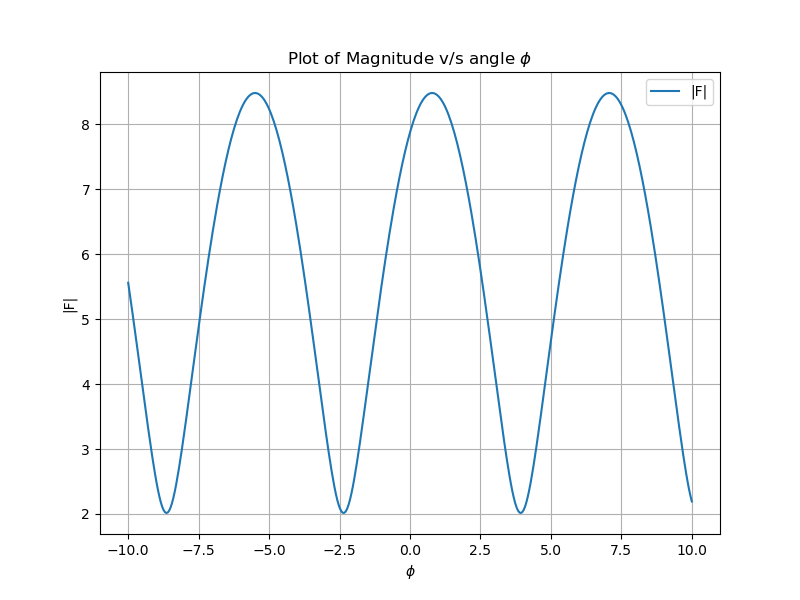
\includegraphics[width=0.8\textwidth]{figs/5a.png}
   % \caption{Electric field lines for the given charge configuration}
    \label{fig:|F|}
\end{figure}

\section{5(b)- Plot of Magnitude of $\vec{F}$ against s}
The code used for this simulation can be found in "codes/5b.py"
\begin{figure}[H]
    \centering
    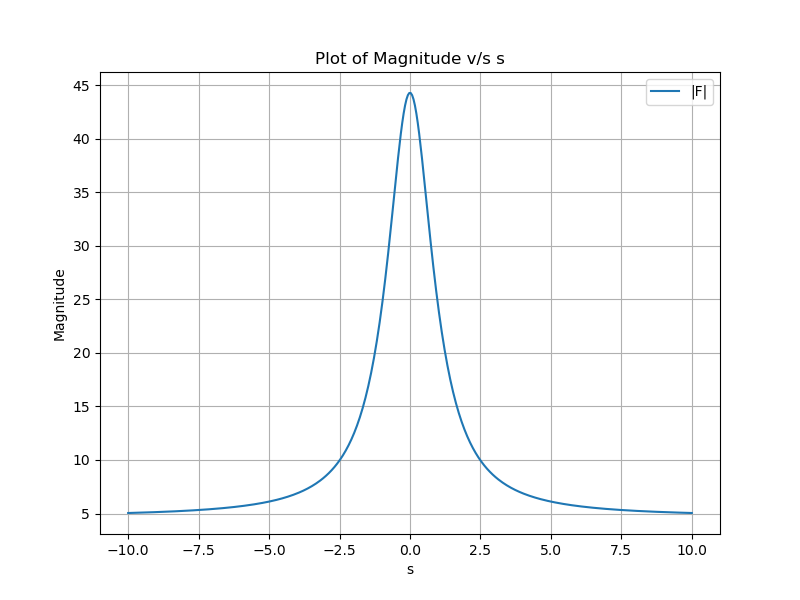
\includegraphics[width=0.8\textwidth]{figs/5b.png}
   % \caption{Electric field lines for the given charge configuration}
    \label{fig:|F|}
\end{figure}

\section{6(a)- Plot of Electric Field}
The code used for this simulation can be found in "codes/6a.py"
\begin{figure}[H]
    \centering
    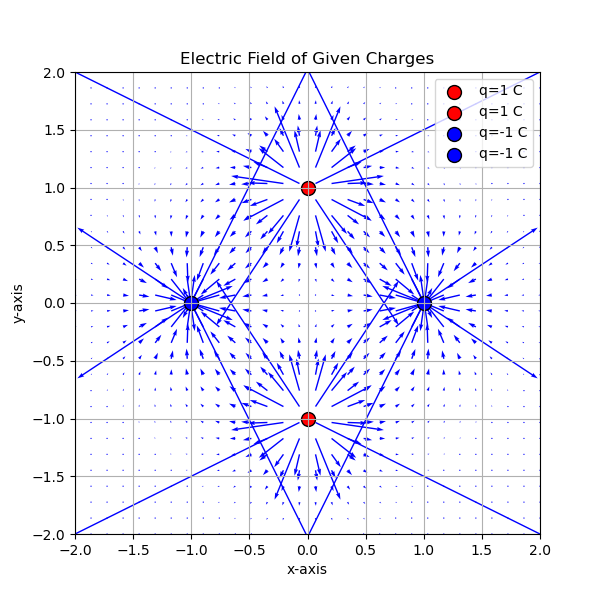
\includegraphics[width=0.8\textwidth]{figs/6a.png}
   % \caption{Electric field lines for the given charge configuration}
    \label{fig:Electric field}
\end{figure}

\section{6(b)- Plot of Electric Potential(along Z-axis)}
The code used for this simulation can be found in "codes/6b.py"
\begin{figure}[H]
    \centering
    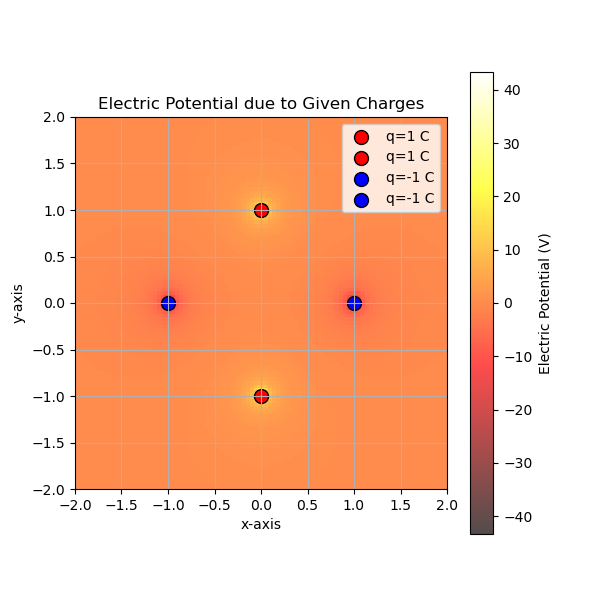
\includegraphics[width=0.8\textwidth]{figs/6b.png}
   % \caption{Electric field lines for the given charge configuration}
    \label{fig:|F|}
\end{figure}

\end{document}

